\documentclass[a4paper,12pt]{article}
\usepackage[utf8]{inputenc}
\usepackage[T1]{fontenc}
\usepackage{graphicx}
\usepackage{enumitem}
\usepackage{geometry}
\usepackage{titling}
\usepackage{parskip}
\usepackage[colorlinks=true, allcolors=blue]{hyperref}
\usepackage{array}
\usepackage{booktabs}
\usepackage{listings}
\usepackage{array}
\usepackage{fancyvrb}
\usepackage[table]{xcolor}
\usepackage{hyperref}
\geometry{margin=2.5cm}

\lstdefinestyle{javascript}{
    language=python,
    basicstyle=\ttfamily\footnotesize,
    keywordstyle=\color{blue},
    commentstyle=\color{green},
    stringstyle=\color{red},
    numbers=left,
    numberstyle=\tiny\color{gray},
    breaklines=true,
    frame=single,
    showspaces=false,
    showstringspaces=false,
    tabsize=2,
    upquote=true,
    columns=fixed,
    basewidth=0.5em
}
\title{Práctica 4: Módulos Odoo Modelo y Vista.}
\author{Andrea Sofía Pais Dos Santos}
\date{\today}

\begin{document}
\setlength{\droptitle}{0.4\textheight} 
\maketitle
\thispagestyle{empty}
\newpage 


\vspace{7cm}

\section{Índice}

\begin{enumerate}[start=2]
    \item Introducción  .............................................................................................. página 3
    \item Actividad 01 - Liga Fútbol ........................................................................ página 3
    \begin{itemize}
    \item Modificar lógica de puntuación de partidos
    \item Botones para alterar goles de los partidos
    \item Web controller para eliminar empates
    \item Informe para cada partido
    \item Wizard para crear nuevos partidos
    \item Vista Graph
    \item Errores encontrados
    \end{itemize}
    \item Actividad 02 - Pruebas Api Rest Socios ................................................... página 8
    \begin{itemize}
    \item Probar crear, modificar, consultar y eliminar
    \item Utilizar una herramienta como: (Postman, Thunder Client)
    \item Errores Encontrados
    \end{itemize}
    \item Actividad 03 - Bot de Telegram conectado a la Api Rest ......................... página 18
    \begin{itemize}
    \item Crear bot de Telegram configurando con BotFather
    \item Escuchar órdenes enviados por los usuarios
    \item El bot tiene que soportar el bot
    \item Errores encontrados 
    \end{itemize}
    \item Actividad 04 -  Generar de imágenes aleatorias con Web Controller ......... página 28
    \begin{itemize}
    \item Crear un Web Controller
    \item Errores encontrados 
    \end{itemize}
    \item Conclusiones ............................................................................................. página 44
\end{enumerate}
\newpage


\section{Introducción}

El objetivo de la práctica es aplicar lo aprendido sobre informes, vistas, wizard y controladores web para seguir adquiriendo conceptos y ser capaces de crear módulos por nuestra cuenta cada vez más complejos. Nos vamos a basar en ejemplos del 01 al 06 del repositorio que nos proporcionan en el enuncionado: \href{https://github.com/sergarb1/OdooModulosEjemplos}{repositorio de ejemplo}.

Hay que tener en cuenta que para ir viendo si funciona los módulos y sus respectivas vistas estén correctos tenemos que levantar el contenedor en docker, iniciar en Odoo con nuestros datos, actualizar la lista de aplicaciones y realizar lo que necesitemos: activar módulo, actualizar módulo, etc.

\section{Actividad 01 - Liga Fútbol}
Para esta activadad importamos el módulo de base que está en el repositorio que se ha dado para la práctica: \href{https://github.com/sergarb1/OdooModulosEjemplos}{repositorio de ejemplo}. Teniendo esta base, levantados el contenedor de docker que teníamos para las anteriores prácticas y iniciamos en Odoo con nuestros datos. Si estamos en modo desarrollador, actualizamos nuestra lista de aplicaciones e instalamos el módulo nuevo "Liga Fútbol".

\begin{center}
    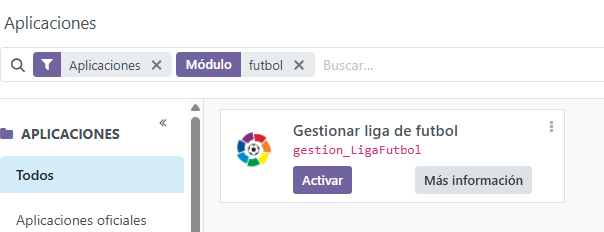
\includegraphics[height=5cm]{images/futbol1png.png}
\end{center}

\subsection{Modificar lógica de puntuación de partidos}
Lo que hay que añadir en este apartado es que si en un partido hay más de 4 goles de diferencia el que gana se le suma 4 puntos y el que pierde -1 punto. Si esa diferencia no existe y no hay un empate, el equipo ganador se sigue llevando 3 puntos y el perdedor 0 puntos. En caso de empate los equipos se llevan 1 punto cada uno.

Para saber si nos va a funcionar el cambio en la lógica, cree dos equipos de fútbol inspirados en la liga de Ourense de 1º FutGal.

\vspace{0.2cm}
\begin{center}
    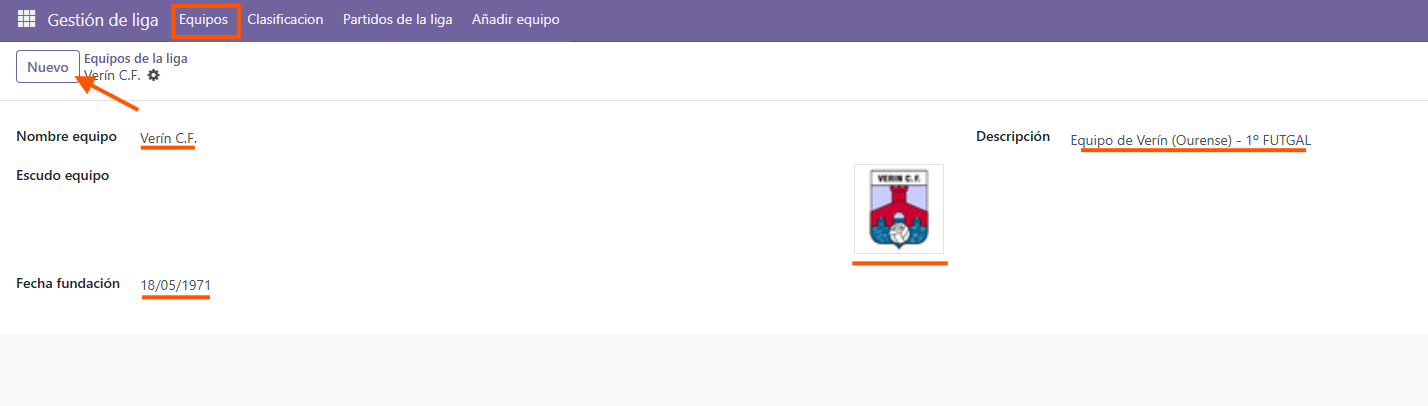
\includegraphics[height=4cm]{images/futbol2.png}
\end{center}

Al tener los 2 equipos, en clasificación vamos a tener todos los datos de los resultados de los partidos y los puntos que tenemos que modificar ahora, porque de momento solo están los puntos de victoria de 3 puntos, de empate 1 punto y de derrota 0 punto.

\vspace{0.2cm}
\begin{center}
    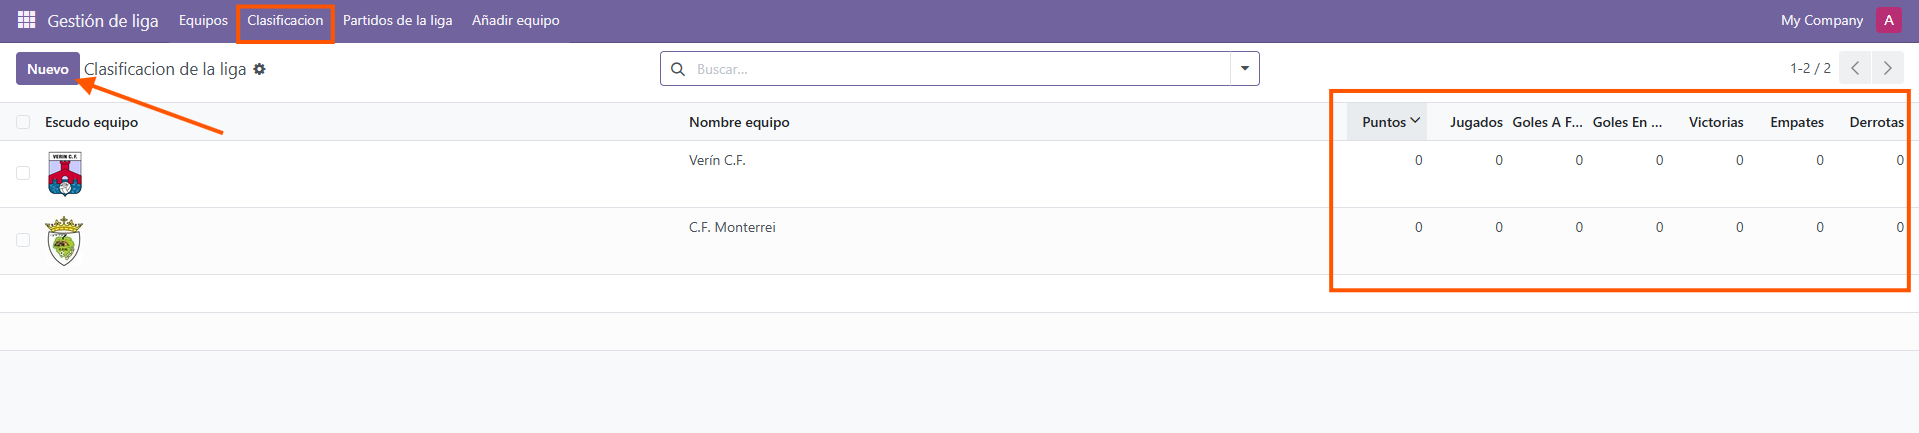
\includegraphics[height=3.5cm]{images/futbol3.png}
\end{center}

Para realizar los cambios que tenemos que hacer, hay que cambiar el archivo models "liga partido". En el documento ya hay una base de como funciona los puntos base.

\vspace{0.5cm}
\begin{lstlisting}[style=javascript]
def actualizoRegistrosEquipo(self):
        #Recorremos partidos y equipos
        for recordEquipo in self.env['liga.equipo'].search([]):
            #Como recalculamos todo, ponemos de cada equipo todo a cero
            recordEquipo.victorias=0
            recordEquipo.empates=0
            recordEquipo.derrotas=0
            recordEquipo.goles_a_favor=0
            recordEquipo.goles_en_contra=0
            recordEquipo.puntos= 0
            
            for recordPartido in self.env['liga.partido'].search([]):  
        
                #Si es el equipo de CASA
                if recordPartido.equipo_casa.nombre == recordEquipo.nombre:
                    
                    #Miramos si es victoria o derrota
                    if recordPartido.goles_casa > recordPartido.goles_fuera:
                        recordEquipo.victorias=recordEquipo.victorias + 1
                        # Si los goles marcados por el equipo de casa es mas de 4 goles por encima del equipo visitante
                        if recordPartido.goles_casa - recordPartido.goles_fuera >= 4:
                            #Se suman los 4 puntos
                            recordEquipo.puntos = recordEquipo.puntos + 4
                        else:
                            #Si no hay esa diferencia se le suma al equipo de casa 3 puntos por victoria
                            recordEquipo.puntos = recordEquipo.puntos + 3
                    elif recordPartido.goles_casa < recordPartido.goles_fuera:
                        recordEquipo.derrotas = recordEquipo.derrotas + 1
                        #Si los goles marcados por el equipo de fuera es mas de 4 goles que el otro equipo, al equipo de casa
                        if recordPartido.goles_fuera - recordPartido.goles_casa >= 4:
                            #Se le resta 1 punto 
                            recordEquipo.puntos = recordEquipo.puntos - 1
                    else:
                        recordEquipo.empates = recordEquipo.empates + 1
                        #Un punto por empate 
                        recordEquipo.puntos = recordEquipo.puntos + 1
                        
                    #Sumamos goles a favor y en contra
                    recordEquipo.goles_a_favor = recordEquipo.goles_a_favor+recordPartido.goles_casa
                    recordEquipo.goles_en_contra = recordEquipo.goles_en_contra+recordPartido.goles_fuera

                #Si es el equipo de FUERA
                if recordPartido.equipo_fuera.nombre==recordEquipo.nombre:
                
                    #Miramos si es victoria o derrota
                    if recordPartido.goles_casa < recordPartido.goles_fuera:
                        recordEquipo.victorias = recordEquipo.victorias + 1
                        # Si los goles marcados por el equipo de fuera es mas de 4 goles por encima del equipo en casa
                        if recordPartido.goles_fuera - recordPartido.goles_casa >= 4:
                            #Se suman los 4 puntos
                            recordEquipo.puntos = recordEquipo.puntos + 4
                        else:
                            #Si no hay esa diferencia se le suma al equipo de casa 3 puntos por victoria
                            recordEquipo.puntos = recordEquipo.puntos + 3
                    elif recordPartido.goles_casa > recordPartido.goles_fuera:
                        recordEquipo.derrotas = recordEquipo.derrotas + 1
                        # Si los goles marcados por el equipo de casa es mas de 4 goles por encima del equipo de fuera
                        if recordPartido.goles_casa - recordPartido.goles_fuera >= 4:
                            # Se le resta 1 punto
                            recordEquipo.puntos = recordEquipo.puntos - 1 
                    else:
                        recordEquipo.empates = recordEquipo.empates + 1
                        #Uno por empate
                        recordEquipo.puntos = recordEquipo.puntos + 1
                    
                    #Sumamos goles a favor y en contra
                    recordEquipo.goles_a_favor = recordEquipo.goles_a_favor + recordPartido.goles_fuera
                    recordEquipo.goles_en_contra = recordEquipo.goles_en_contra + recordPartido.goles_casa
\end{lstlisting}

Como base ya viene una estructura que añade 3 puntos por victoria y los puntos por empate y partido perdido. Lo que nos pide es añadir al equipo ganador sea de casa o visitante y los goles son superior a 4 goles del rival hay que sumarle +4 puntos al equipo ganador.

\vspace{1.5cm}
\subsection{Botones para alterar goles de los partidos}
El objetivo de este apartado es crear dos botones que sumen goles de 2 en 2 por un lado a los equipos locales y también a los visitantes. Luego se tiene que recalcular la clasificación.

Lo primero es en el archivo "liga partido.py" añadimos las funciones que harán que cambien los goles y aumenten según que equipo sea.

\vspace{0.5cm}
\begin{lstlisting}[style=javascript]
    # Sumar los 2 goles a los equipos locales
    def sumar_goles_locales(self):
        #Buscar todos los partidos
        partidos = self.search([])
        for partido in partidos:
            partido.goles_casa += 2
        self.actualizoRegistrosEquipo()
        return True
    
    # Sumar los 2 goles a los equipos visitantes
    def sumar_goles_visitantes(self):
        #Buscar todos los partidos
        partidos = self.search([])
        for partido in partidos:
            partido.goles_fuera += 2
        self.actualizoRegistrosEquipo()
        return True

\end{lstlisting}

Lo complicado era crear los botones en la vista, porque en la vista Kanban los botones se añadían dentro de la tarjeta y tenía que modificar todos los equipos. 
La manera de solucionarlo para que los botones aparezca arriba en ambas vistas es meterlo dentro de la etiqueta "header" que en lista no funciona a no ser que se le añada display="always".

\vspace{0.5cm}
\begin{lstlisting}[style=javascript]
    <!-- Vista List -->
    <record id="liga_partido_view_list_nueva" model="ir.ui.view">
        <field name="name">Lista de partidos de la liga</field>
        <field name="model">liga.partido</field>
        <field name="arch" type="xml">
            <list>
                <header>
                    <button name="sumar_goles_locales" string="+2 Goles Locales" type="object" display="always"/>
                    <button name="sumar_goles_visitantes" string="+2 Goles Visitantes" type="object" display="always"/>
                </header>
                <!-- Indicamos que atributos usaremos al hacer la vista List -->
                <field name="equipo_casa" />
                <field name="goles_casa" />
                <field name="equipo_fuera" />
                <field name="goles_fuera" />
            </list>
        </field>
    </record>
    <!-- Y lo mismo en la vista kanban -->
    <record id="liga_partido_view_kanban" model="ir.ui.view">
        <field name="name">Lista de partidos de la liga</field>
        <field name="model">liga.partido</field>
        <field name="arch" type="xml">
            <!-- Agrupamos por el atributo "parent_id"-->
            <kanban>
                <!-- Indicamos que atributos usaremos al hacer la vista Kanban -->
                <header>
                    <button name="sumar_goles_locales" string="+2 Goles Locales" type="object" display="always"/>
                    <button name="sumar_goles_visitantes" string="+2 Goles Visitantes" type="object" display="always"/>
                </header>
                <field name="equipo_casa" />
                <field name="goles_casa" />
                <field name="equipo_fuera" />
                <field name="goles_fuera" />
                ...


\end{lstlisting}

Por lo que visualmente quedaría así los botones de sumar goles:

\vspace{0.2cm}
\begin{center}
    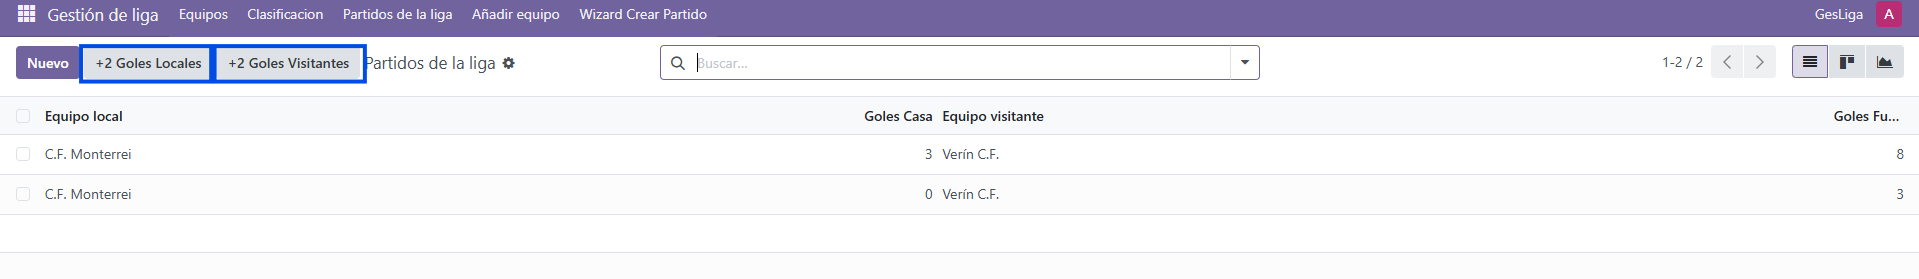
\includegraphics[height=2.3cm]{images/futbol18.png}
\end{center}

Así quedaría si sumamos 2 goles a los equipos locales y dos a los visitantes.

\vspace{0.2cm}
\begin{center}
    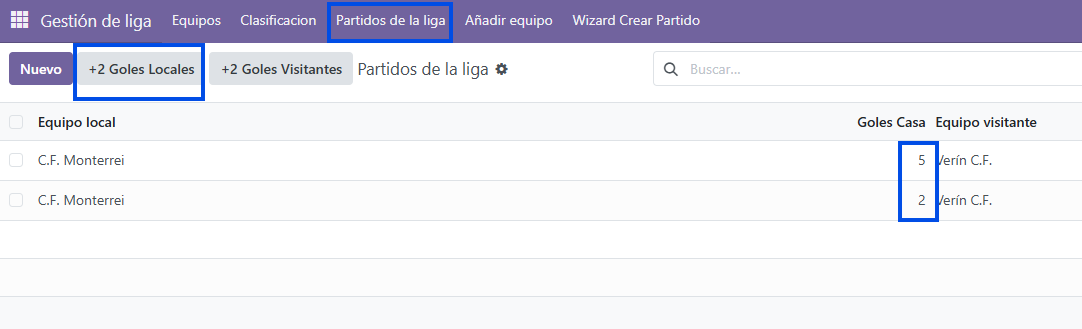
\includegraphics[height=4cm]{images/futbol19.png}
\end{center}

\vspace{0.5cm}
\subsection{Web controller para eliminar empates}
Para crear un Web Controller vamos a necesitar crear en el módulo un carpeta "controllers" que necesita un archivo "init" y un archivo "main". Como cogimos como base el que está en el repositorio ya está creado. Ahora lo que vamos es a editar el archivo "main".

\vspace{0.5cm}
\begin{lstlisting}[style=javascript]
    #Al acceder a http://localhost:8069/eliminarempates borra los partidos empatados
    @http.route("/eliminarempates",type="http",auth="public", website=True)
    def eliminar_empates(self,**kw):
        #Buscamos los partidos
        partidos = request.env["liga.partido"].sudo().search([])
        #Empezamos un contador
        contador = 0
        #Buscamos que partidos tiene los goles iguales
        for partido in partidos:
            if partido.goles_casa == partido.goles_fuera:
                #Borrar los registros
                partido.unlink()
                #Vamos sumando los partidos empatados borrados
                contador += 1
        request.env["liga.partido"].sudo().actualizoRegistrosEquipo()
        #Nos devuelve unos textos que nos dice cuantos partidos se borrar con empates
        return "<h1>Operacion realizada</h1><p>Se han borrado un total de partidos con empate: %s</p>" % contador
\end{lstlisting}

Ahora para probarlo actualizamos el módulo, creamos un partido con goles empatados y entramos en la url http://localhost:8069/eliminarempates. 

\vspace{0.2cm}
\begin{center}
    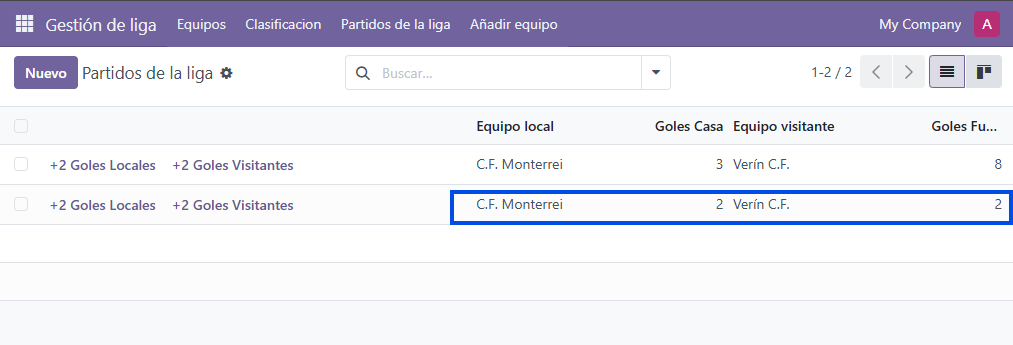
\includegraphics[height=4.8cm]{images/futbol9.png}
\end{center}

Al entrar en la ruta vemos que se ha eliminado el partido empatado.

\vspace{0.2cm}
\begin{center}
    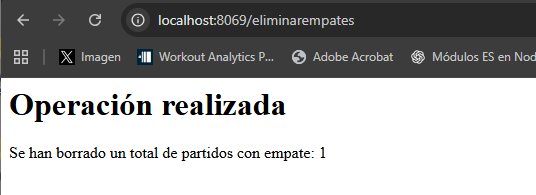
\includegraphics[height=4.8cm]{images/futbol10.png}
\end{center}

Para ver que se borró volvemos a la lista de partidos y vemos que ya se ha borrado el partido.

\vspace{0.2cm}
\begin{center}
    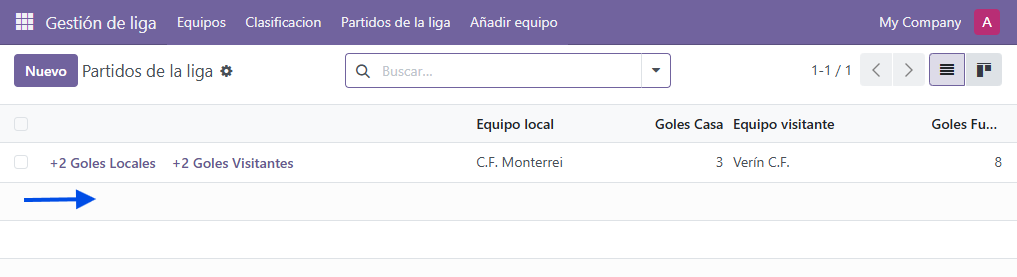
\includegraphics[height=4.3cm]{images/futbol11.png}
\end{center}

\vspace{0.5cm}
\subsection{Informe para cada partido}
Para generar un informe de cada partido hay que crear un botón para impirmir el informe y nos lo genere y una plantilla de como se verá visualmente el informe. 
En vistas creo una nueva vista "liga partido informe" y la diseñamos con todos los datos principales que necesitan un informe.

\vspace{0.5cm}
\begin{lstlisting}[style=javascript]
    <?xml version="1.0" encoding="utf-8"?>
<odoo>
    <!--Tienen que estar los atributos en ingles-->
    <record id="action_report_partido" model="ir.actions.report">
        <field name="name">Resultado del Partido</field>
        <field name="model">liga.partido</field>
        <field name="report_type">qweb-pdf</field>
        <field name="report_name">gestion_LigaFutbol.informe_partido_plantilla</field>
        <field name="print_report_name">'Partido -- %s' % (object.equipo_casa.nombre)</field>
        <field name="binding_model_id" ref="model_liga_partido"/>
        <field name="binding_type">report</field>
    </record>

    <template id="informe_partido_plantilla">
        <t t-call="web.html_container">
            <t t-foreach="docs" t-as="o">
                <t t-call="web.external_layout">
                    <div class="datos">
                        <!--Datos de los equipos -->
                        <div class="datos2">
                            <p>EQUIPO LOCAL</p>
                            <p t-field="o.equipo_casa.nombre"></p>
                        </div>
                        <div class="datos2">
                            <p>EQUIPO VISITANTE</p>
                            <p t-field="o.equipo_fuera.nombre"></p>
                        </div>
                    </div>
                    <!--resultado del partido con goles-->
                    <div class="pagina">
                        <div class="text-center" style="border-bottom: 2px solid black; margin-bottom: 20px;">
                            <h2>ACTA DEL PARTIDO</h2>
                        </div>
                        
                        <div class="row align-items-center justify-content-center" style="font-size: 20px; margin-top: 50px;">
                            <div class="col-5 text-end"> <strong t-field="o.equipo_casa.nombre"/>
                            </div>
                            
                            <div class="col-2 text-center" style="background-color: #f2f2f2; border-radius: 10px; width: 100px; padding: 10px; margin-left: 5px; margin-right: 5px;">
                                <strong>
                                    <span t-field="o.goles_casa"/> - <span t-field="o.goles_fuera"/>
                                </strong>
                            </div>
                            
                            <div class="col-5 text-start"> <strong t-field="o.equipo_fuera.nombre"/>
                            </div>
                        </div>
                        <!--Pie de acta que sino quedaba muy vacio-->
                        <div class="text-center" style="margin-top: 100px; color: grey;">
                            <p>Informe generado por el Sistema de Gestion de la Liga</p>
                        </div>
                    </div>
                </t>
            </t>
        </t>
    </template>
</odoo>
\end{lstlisting}

Además hay que añadir al archivo manifest principal del módulo en "data" la nueva vista creada: 

\vspace{0.5cm}
\begin{lstlisting}[style=javascript]
    'data': [
        #'security/groups.xml',
        'security/ir.model.access.csv',

        #Aqui distintas vistas de equipo (vistas diferentes, mismo modelo)
        'views/liga_equipo.xml',
        'views/liga_equipo_clasificacion.xml',
        #Vista a un informe
        'report/liga_equipo_clasificacion_report.xml',
        #Aqui vista sobre los partidos
        'views/liga_partido.xml',
        'wizard/liga_equipo_wizard.xml',
        # Poner la nueva vista
        'views/liga_partido_informe.xml'
        
    ],
\end{lstlisting}

Tras diseñar la plantilla del informe para probarlo hay que actualizar el módulo y en el apartado de partido, seleccionamos el partido del que necesitamos el informe y en el icono de ajustes aparece un apartado que es "Resultado del Partido". 

\vspace{0.2cm}
\begin{center}
    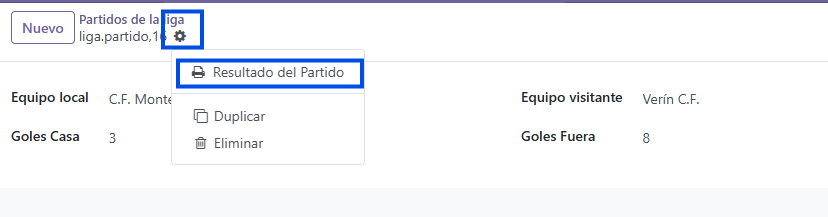
\includegraphics[height=4cm]{images/futbol13.png}
\end{center}

Genera un pdf que se abre automáticamente con los datos del partido.

\vspace{0.2cm}
\begin{center}
    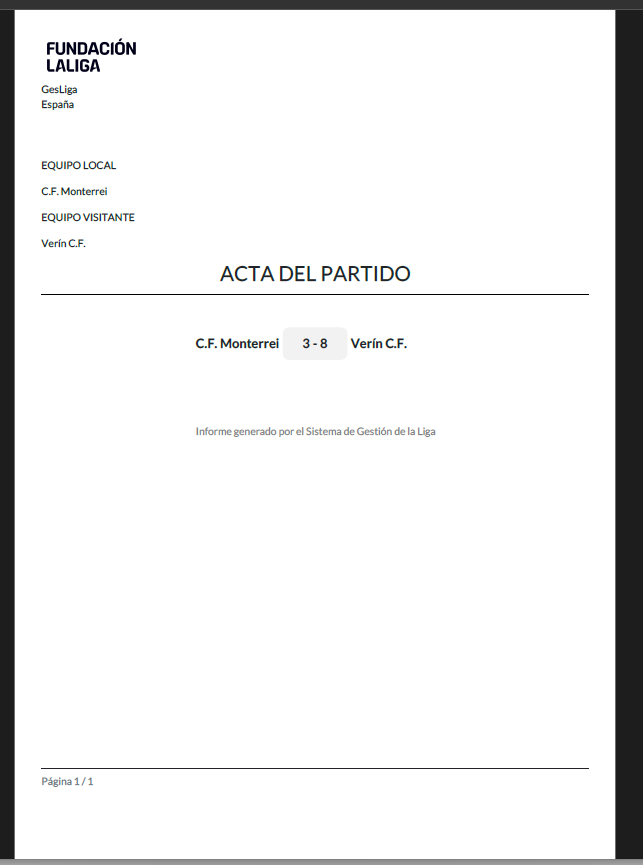
\includegraphics[height=15cm]{images/futbol12.png}
\end{center}

\vspace{0.5cm}
\subsection{Wizard para crear nuevos partidos}
El objetivo de este apartado es crear un partido mediante un formulario emergente que guarda datos temporales. Para crear un Wizard hay que generar un modelo nuevo "partido wizard".

\vspace{0.5cm}
\begin{lstlisting}[style=javascript]
    # -*- coding: utf-8 -*-
    from odoo import models, fields

    class PartidoWizard(models.TransientModel):
        #Nombre de la tabla temporal que se va a crear
        _name = 'liga.partido.wizard'
        _description = 'Wizard para crear partidos'
        #Campos del formulario 
        equipo_casa = fields.Many2one('liga.equipo', string="Equipo Local", required=True)
        equipo_fuera = fields.Many2one('liga.equipo', string="Equipo Visitante", required=True)
        goles_casa = fields.Integer(string="Goles Local", default=0)
        goles_fuera = fields.Integer(string="Goles Visitante", default=0)

        def crear_partido(self):
            # Esta funcion crea el registro permanente en el modelo liga.partido
            self.env['liga.partido'].create({
                'equipo_casa': self.equipo_casa.id,
                'equipo_fuera': self.equipo_fuera.id,
                'goles_casa': self.goles_casa,
                'goles_fuera': self.goles_fuera,
            })
            # Recalcular la clasificacion tras poner el partido nuevo
            self.env['liga.partido'].actualizarRegistrosEquipo()
            return {'type': 'ir.actions.act_window_close'} # Cierra la ventana emergente 
\end{lstlisting}

Ahora hay que hacer una vista para que se genere el formulario anterior "partido wizard vista"

\vspace{0.5cm}
\begin{lstlisting}[style=javascript]
<?xml version="1.0" encoding="utf-8"?>
<odoo>
    <record id="partido_wizard_vista" model="ir.ui.view">
        <field name="name">liga.partido.wizard.form</field>
        <field name="model">liga.partido.wizard</field>
        <field name="arch" type="xml">
            <form string="Crear Nuevo Partido">
                <group>
                    <group>
                        <field name="equipo_casa"/>
                        <field name="goles_casa"/>
                    </group>
                    <group>
                        <field name="equipo_fuera"/>
                        <field name="goles_fuera"/>
                    </group>
                </group>
                <group>
                    <button name="crear_partido" string="Generar Partido" type="object" />
                    <button string="Cancelar" special="cancel"/>
                </group>
            </form>
        </field>
    </record>

    <record id="action_partido_wizard" model="ir.actions.act_window">
        <field name="name">Anadir Partido</field>
        <field name="res_model">liga.partido.wizard</field>
        <field name="view_mode">form</field>
        <field name="target">new</field> 
    </record>

    <menuitem id="menu_partido_wizard" 
              name="Wizard Crear Partido" 
              parent="liga_base_menu" 
              action="action_partido_wizard" 
              sequence="50"/>
</odoo>
\end{lstlisting}

Hay que tener en cuenta que al crear estos archivos ahora en "init" y "manifest" hay que añadir esto nuevo:

En el archivo "init" de la carpeta vista: 
\vspace{0.5cm}
\begin{lstlisting}[style=javascript]
    from . import partido_wizard
\end{lstlisting}

En el archivo "manifest" en data:
\vspace{0.5cm}
\begin{lstlisting}[style=javascript]
    'views/partido_wizard_vista.xml'
\end{lstlisting}

Un error que tuve fue que no me cargaba la vista y tenía que añadir los permisos al archivo "ir.model.access.csv"

\vspace{0.5cm}
\begin{lstlisting}[style=javascript]
    acl_partido_wizard_vista,liga.equipo_wizard,model_partido_wizard,,1,1,1,1
\end{lstlisting}
 
Aquí vemos que nos sale el apartado nuevo arriba en el menú que al pinchar nos abre una ventana emergente para añadir los datos del partido de forma rápida.

\vspace{0.2cm}
\begin{center}
    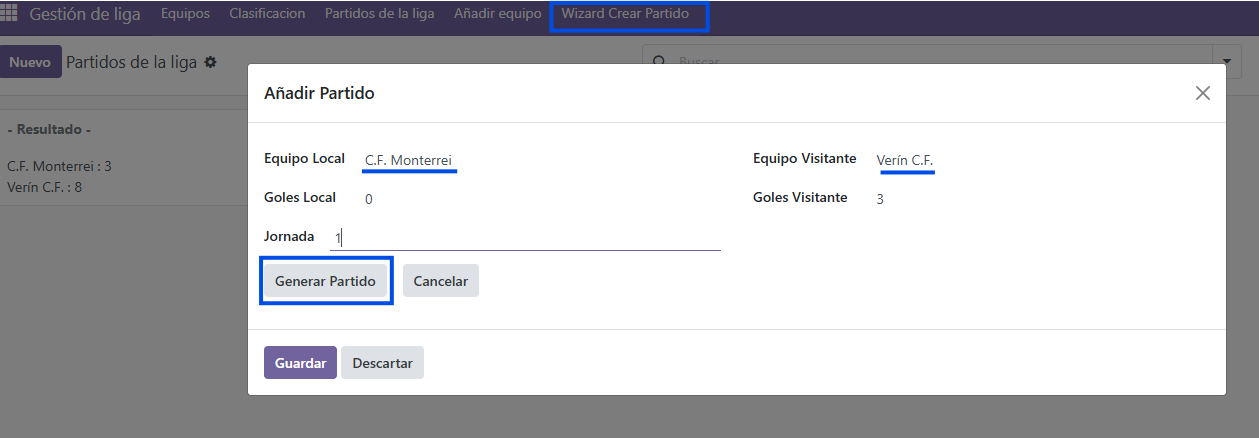
\includegraphics[height=5cm]{images/futbol14.png}
\end{center}

Y ya dentro de los partidos nos sale el que he creado.

\vspace{0.2cm}
\begin{center}
    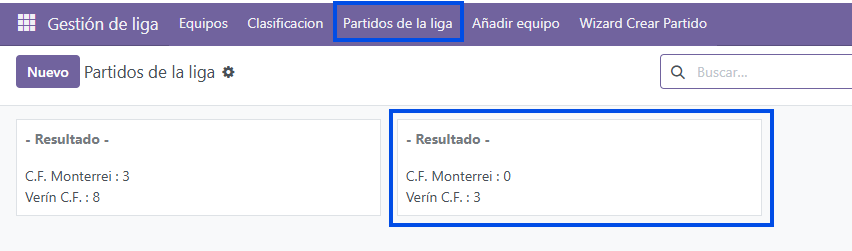
\includegraphics[height=4.3cm]{images/futbol15.png}
\end{center}


\vspace{2cm}
\subsection{Vista Graph}

Para crear una gráfica me basé en la gráfica que estaba en el apartado de equipos y cambié los valores a goles y equipos locales.
Además hay que añadir el parámetro "graph". 

\vspace{0.5cm}
\begin{lstlisting}[style=javascript]
    ...
    <field name="view_mode">list,kanban,form,graph</field>
    ...
    <!-- Vista Graph  que muestra informacion de los goles locales en total-->
    <record model="ir.ui.view" id="liga_partido_view_graph">
        <field name="name">Goles de los equipos locales</field>
        <field name="model">liga.partido</field>
        <field name="type">graph</field>
        <field name="arch" type="xml">
            <!-- Cada fila es un equipo y la altura los goles -->
              <graph string="Puntos por equipo">
                <field name="equipo_casa" group="True" type="row"/>
                <field name="goles_casa" group="True" type="measure"/>
             </graph>
         </field>
     </record>
\end{lstlisting}
 
Ahora para ver la gráfica actualizamos el módulo y dentro del apartado de partidos vemos una nueva vista. Y se ve una gráfica de los equipos locales con los goles totales.

\vspace{1cm}
\begin{center}
    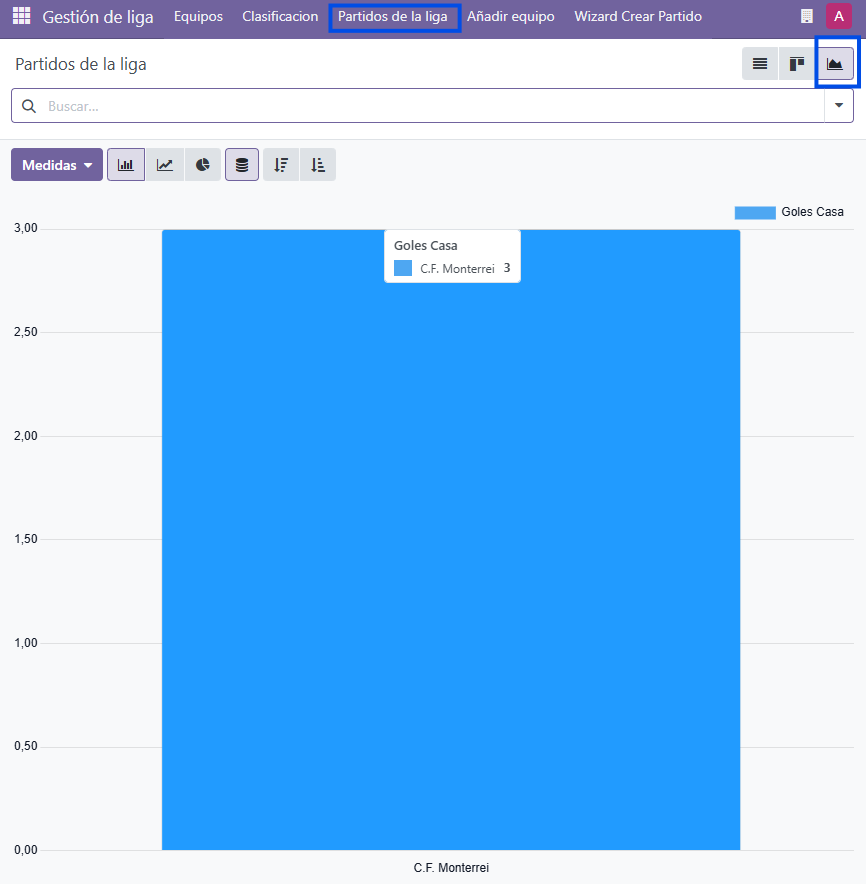
\includegraphics[height=12cm]{images/futbol16.png}
\end{center}

\vspace{0.5cm}
\subsection{Errores encontrados}
El primer error que se tuvo en esta actividad fue al intentar abrir el módulo nos daba un error que ya tuvimos en otras prácticas que era la utilización de la etiqueta <tree> que ya no se utiliza y hay que cambiarlo por <list>. se cambió en todos los archivos de las vistas y el módulo ya se puede abrir correctamente.

Otro error que sucede mucho es equivocarme al llamar con el nombre correcto funciones que creo por ejemplo me dio error en el controlador porque había llamado mal a la función de recargar. 

\vspace{1cm}
\section{Actividad 02 - Pruebas Api Rest Socios}

La actividad 2 consiste en realizar las 4 operaciones básicas (crear, modificar, listar y eliminar) usando en mi caso Thunder Client y ser capaz de ver los resultados en Odoo. La pruebas realizadas se encuentran en este vídeo de youtube \href{https://youtu.be/wQ1JUA7Oems}{pinchar aquí}.

\vspace{1cm}
\begin{center}
    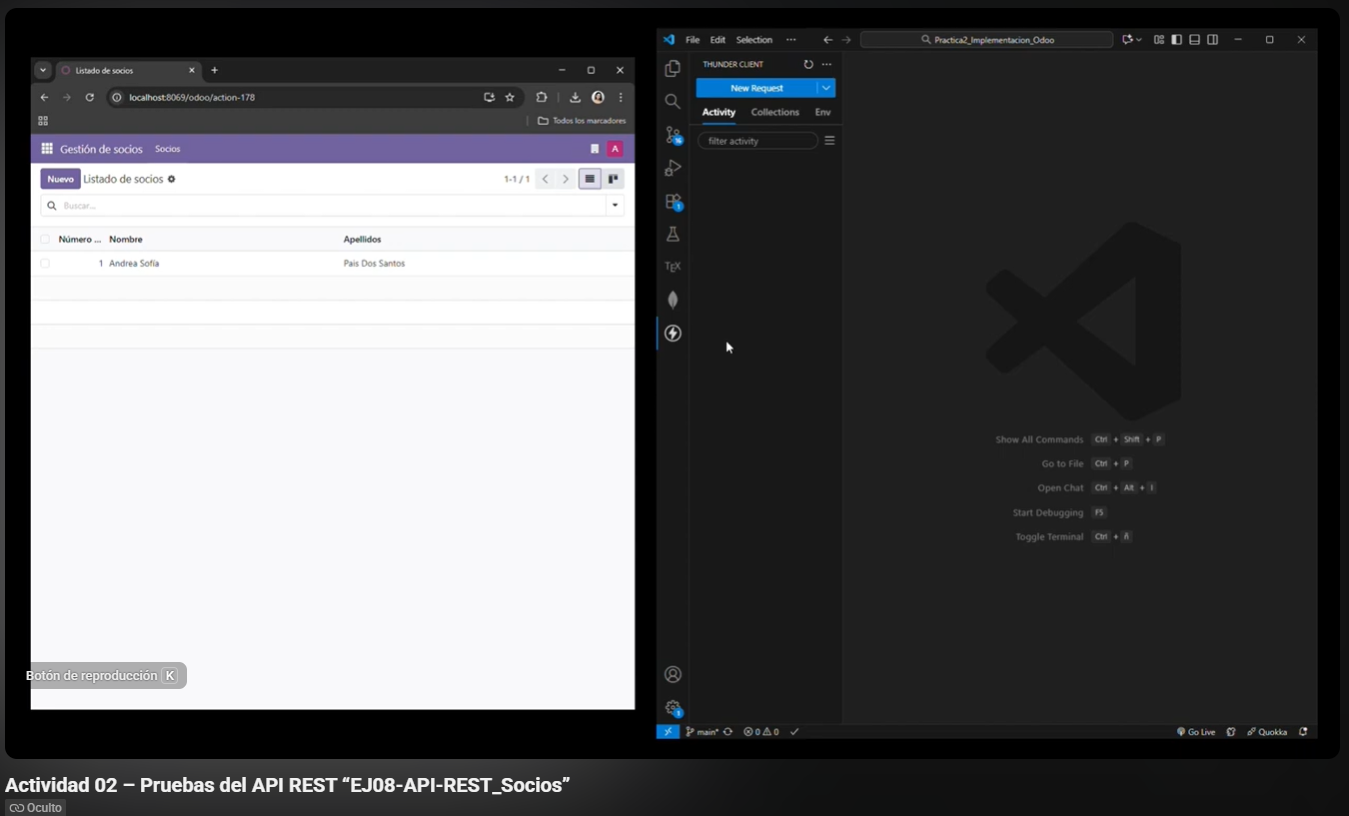
\includegraphics[height=9cm]{images/actividad2.png}
\end{center}

\vspace{1cm}
\section{Actividad 03 - Bot de Telegram conectado a la Api Rest}

En esta actividad vamos a crear primero un bot de Telegram que se va a configurar con BotFather. 

\vspace{0.5cm}
\begin{center}
    
\includegraphics[height=5cm]{images/bot1.png}
\end{center}


\vspace{1cm}
\section{Actividad 04 -  Generar de imágenes aleatorias con Web Controller}

Para esta activadad nos vamos a basar en el módulo 9 del repositorio aportado. Con esa base primero vamos a instalar la librería Pillow en el entorno de Python usando el comando "python -m pip install Pillow".

\vspace{0.5cm}
\begin{center}
    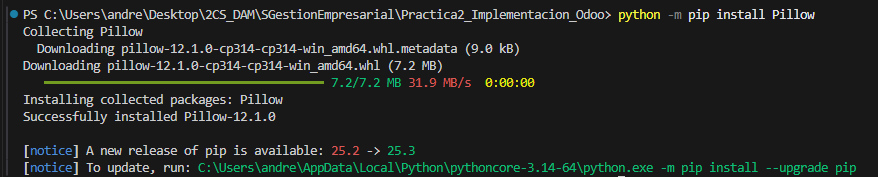
\includegraphics[height=3cm]{images/futbol17.png}
\end{center}

Ahora creamos en la carpeta "controllers" y nuevo archivo "controlador" que se encargará de generar la imagen utiliza la librerá de procesamiento de imágenes Pillow para crear una representación visual de datos aleatorios. 

\vspace{0.5cm}
\begin{lstlisting}[style=javascript]
    # -*- coding: utf-8 -*-
    from odoo import http
    from odoo.http import request
    import io
    import random

    # Intentar importar Pillow de forma segura
    try:
        from PIL import Image
    except ImportError:
        Image = None

    class ImagenAleatoriaController(http.Controller):

        @http.route('/generar_imagen_aleatoria', type='http', auth='public', website=True)
        def crear_imagen(self, w=200, h=200, **kwargs):
            # Si Pillow no esta, se devuelve texto para no dar Error 500
            if Image is None:
                return "Error: La libreria Pillow no esta instalada en el contenedor Odoo."

            try:
                ancho = int(w)
                alto = int(h)
            except:
                ancho, alto = 200, 200

            # Crear la imagen aleatoria
            img = Image.new('RGB', (ancho, alto))
            pixeles = img.load()
            for x in range(ancho):
                for y in range(alto):
                    pixeles[x, y] = (random.randint(0, 255), random.randint(0, 255), random.randint(0, 255))

            # Guardar imagen en buffer
            output = io.BytesIO()
            img.save(output, format="PNG")
            contenido = output.getvalue()
            output.close()

            # Retornar respuesta simple para evitar descargas
            return request.make_response(contenido, [
                ('Content-Type', 'image/png'),
                ('Content-Disposition', 'inline')
            ])
\end{lstlisting}

En el archivo "init" del módulo hay que importar el controler y para probarlo vamos a actualizar el módulo primero y luego con la url accedemos al generador de imagen: \href{http://localhost:8069/generar_imagen_aleatoria?w=600&h=600}{generar imagen}.

\vspace{0.5cm}
\begin{center}
    
\includegraphics[height=9cm]{images/pixel1.png}
\end{center}


\vspace{1cm}
\section{Conclusiones}

Al empezar la práctica fue bastante confuso por donde empezar y organizarse de la manera más óptima para realizar correctamente el módulo. Fue todo prueba y error en los 2 primeros ejercicios. Aunque al empezar a realizar las otras actividades se veía un patrón de como es mejor realizar el módulo y como documentarlo de la mejor mamera.

Poco a poco, se hacía algo más "ameno" podía reciclar las bases de los modelos y los módulos y a la vez empezaba a ver más facilmente donde fallaba y más cuando eran errores tontos de palabras mal escritas que fue lo que más rabia me dio de la actividad. He perdido mucho tiempo por olvidarme de como había nombrado atribulos en los modelos y luego en las vistas ponía yo otra que pensaba que era esa y no lo era. 

En conclusión, fue un trabajo bastante largo pero la verdad es que aprendí bastante en poco tiempo como estructurar los módulos correctamente e ir comprobando que todo funcione correctamente.


\end{document}